% ============================================================
%  Think with Images, Learn from Failure:
%  Training-Free Self-Evolution of Visual Agents
%  via Skill and Tool Generation
%
%  Target venue: *ACL submission  |  Page budget: 8 pages (main content)
% ============================================================

% Pass xcolor options before documentclass to avoid option clash
\PassOptionsToPackage{table}{xcolor}

\documentclass[11pt]{article}
\usepackage[review]{acl}

\usepackage{times}
\usepackage{latexsym}
\usepackage[T1]{fontenc}
\usepackage[utf8]{inputenc}
\usepackage{microtype}
\usepackage{inconsolata}

% Provide \laplace before math_commands.tex attempts \renewcommand
\providecommand{\laplace}{\mathcal{L}}

% Math & notation
\input{math_commands.tex}

% Standard packages
\usepackage{url}
\usepackage{xurl}
\usepackage{booktabs}
\usepackage{graphicx}
\usepackage{subcaption}
\usepackage{amssymb}
\usepackage{amsmath,amsfonts}
\usepackage[most]{tcolorbox}
\tcbuselibrary{breakable}
\usepackage{siunitx}
\usepackage{colortbl}
\usepackage{color}
\usepackage{wrapfig}
\usepackage{array}
\usepackage{textcomp}
\usepackage{stfloats}
\usepackage{float}
\usepackage{verbatim}
\usepackage{listings}
\usepackage[ruled, linesnumbered, lined]{algorithm2e}
\usepackage{multirow}
\usepackage{enumitem}
\usepackage{pifont}       % for \ding{51} / \ding{55} checkmarks
\usepackage{etoolbox}
\usepackage[normalem]{ulem}
% Note: xcolor already loaded via \PassOptionsToPackage above

% ---- Colour definitions ----
\definecolor{BestColor}{HTML}{C8E6C9}
\definecolor{SecondBestColor}{HTML}{FFF9C4}
\definecolor{impcolor}{HTML}{2E8B57}
\definecolor{mygray}{gray}{0.9}

\lstdefinestyle{appendixsnippet}{
  basicstyle=\ttfamily\scriptsize,
  breaklines=true,
  breakatwhitespace=true,
  columns=fullflexible,
  keepspaces=true,
  showstringspaces=false
}

% ---- Table helpers ----
\newcommand{\best}[1]{\cellcolor{BestColor}\textbf{#1}}
\newcommand{\secondbest}[1]{\cellcolor{SecondBestColor}#1}

% ---- Inline colour helpers ----
\def\rr{\textcolor{red}}
\def\bb{\textcolor{blue}}

% ---- Agent / notation macros ----
% Change \sysname to your preferred system name before submission
\newcommand{\sysname}{\textsc{DYNAMO}}

% Paper-specific math notation
\newcommand{\Dtrain}{\mathcal{D}_{\text{train}}}
\newcommand{\Dval}{\mathcal{D}_{\text{val}}}
\newcommand{\capset}{\mathcal{C}}
\newcommand{\Skills}{\mathcal{S}}
\newcommand{\Tools}{\mathcal{T}}

% tcolorbox style for example boxes
\newtcolorbox{examplebox}[2][]{
  breakable, enhanced,
  colback=white, colframe=cyan, coltitle=white,
  fonttitle=\bfseries, title=#2,
  overlay middle={\draw[cyan, line width=1pt](frame.south west)--(frame.south east);},
  overlay last={\draw[cyan, line width=1pt](frame.south west)--(frame.south east);},
  #1
}

% ---- Improvement score helpers ----
\newcommand{\improvementstyle}[1]{$^{\textcolor{impcolor}{\tiny #1}}$}
\newcommand{\scoreimp}[2]{%
  \textbf{#1}%
  \ifstrequal{#2}{+0.0}{}{%
    \ifstrequal{#2}{0.0}{}{%
      \makebox[0pt][l]{\improvementstyle{#2}}%
    }%
  }%
}
\newcommand{\scorebase}[1]{#1}

% ============================================================
%  Title, authors (anonymous for submission)
% ============================================================
\title{DYNAMO: Dynamic Skill-Tool Evolution for Vision-Language Agents}

% Anonymous submission; the ACL review option replaces this with an anonymous header.
\author{Anonymous ACL submission}

% ============================================================
%  Abstract
% ============================================================

\begin{document}
\maketitle

\begin{abstract}
Vision-language models (VLMs) remain brittle on visual reasoning, and improving them
typically requires retraining or hand-designed prompts and tools. We present \sysname{},
a training-free framework in which a frozen VLM agent acquires reusable capabilities from
a small training subset. \sysname{} samples a sub-training set, diagnoses \emph{both}
correct and incorrect attempts---using the original images, intermediate tool outputs, and
reasoning traces---and an evolution planner decides whether each missing capability is
\emph{cognitive} (a reusable reasoning skill) or \emph{perceptual} (an executable visual
tool). The Generator proposes multiple candidate skill$+$tool combinations; validation on
the training subset selects the best, and a mastery phase further learns when each tool is
safe to deploy. Promoted capabilities accumulate in a persistent library without any
weight updates. Across ChartQA, MathVista, HRBench, and V$^*$ on six foundation models,
skill-tool co-evolution improves direct inference in 21 of 23 model--benchmark settings,
averaging $+4.8$ accuracy points. On the GTA benchmark, mastery profiling improves
step-level tool selection, argument, and instruction-following accuracy across all tested
backbones. Compared with task-specific RL (VTool-R1, DeepEyes), \sysname{} closes
60--94\% of the gap on chart and table reasoning without any gradient updates, and at 7B
matches DeepEyes on V$^*$ (91.1 vs.\ 90.1). These results suggest that capability evolution
is a viable training-free alternative to task-specific RL.
\end{abstract}

% ---- Main sections ----
\section{Introduction}
% ============================================================
%  §1  Introduction
% ============================================================

Vision-language models (VLMs) have improved rapidly, yet adapting a VLM to a new
visual-reasoning task family still typically requires manually curated SFT data or a
hand-designed RL pipeline---per task and per backbone. We ask whether the agent can build
its own task-family-specific capability set instead, by inspecting its own behaviour on a
small training subset and without any weight updates. We illustrate this motivation in
Figure~\ref{fig:motivation}.

\begin{figure}[t]
  \centering
  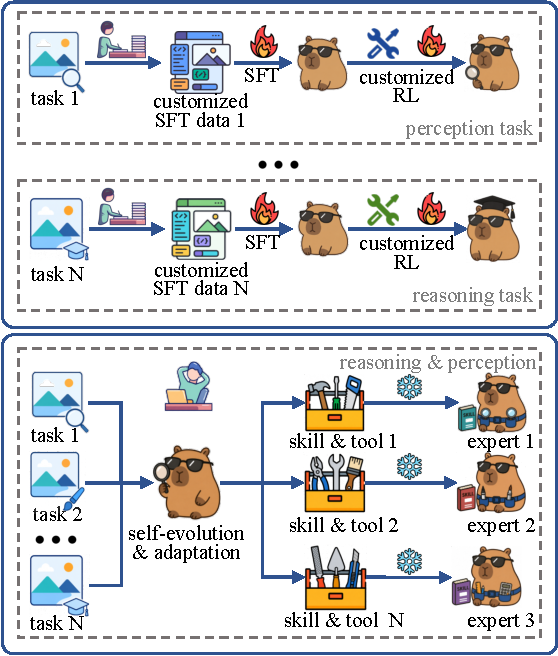
\includegraphics[width=\columnwidth]{figures/Picture2.pdf}
  \caption{
    \textbf{Per-task adaptation without weight updates or hand-authored prompts.}
    Per-task VLM adaptation typically requires manually curated SFT data with a
    hand-designed RL pipeline for every new task family. \sysname{} instead lets a frozen
    VLM agent evolve its own skill and tool set per task family from a small labeled
    training subset---without any weight updates or hand-authored task-specific
    prompts---and dynamically equips the matching set when a case from that family arrives.
  }
  \label{fig:motivation}
\end{figure}

We instantiate this idea in \sysname{}, a training-free framework that evolves two
complementary capability types from a small labeled training subset and dynamically
equips them at inference. \textbf{Skills} are
structured Markdown SOPs for \emph{cognitive} bottlenecks, where the visual evidence is
available but the agent's reasoning procedure is weak. \textbf{Tools} are short Python
programs for \emph{perceptual} bottlenecks, where the agent needs a transformed view---a
crop, zoom, contrast adjustment, or rerendering---before the evidence becomes legible. On
each iteration over a sampled sub-training set, \sysname{} diagnoses both the correct and
the incorrect attempts using their images and reasoning traces, proposes multiple candidate
skill$+$tool combinations, and promotes the highest-validation-accuracy candidate into a
persistent library. A mastery phase further learns when each tool is safe to invoke, so
that promoted capabilities are deployed selectively rather than indiscriminately.

We evaluate three questions.
\textbf{(I) Does \sysname{} work across diverse benchmarks and backbones?}
On ChartQA, MathVista, HRBench, and V$^*$ across six VLM backbones, skill-tool co-evolution
improves direct inference on all 20 model--benchmark settings, averaging $+4.7$ accuracy
points.
\textbf{(II) Does the framework extend to a tool-mastery setting with a curated tool set?}
On GTA, mastery profiling lifts step-level tool selection, argument, and instruction-following
accuracy across all tested backbones.
\textbf{(III) Can \sysname{} match task-specific RL across different task families?}
Across three task families---chart, table, and high-resolution perception---we compare
\sysname{} to a representative RL method on each (VTool-R1 for chart/table;
DeepEyes for perception). \sysname{} matches or approaches RL accuracy at a fraction of
the compute (60--94\% gap recovery on chart/table; 91.1 vs.\ 90.1 on V$^*$-7B perception),
and combines additively with RL when both are available.

\paragraph{Contributions.}
\begin{enumerate}[leftmargin=*, label=(\arabic*), noitemsep]
  \item A \textbf{problem formulation} that recasts per-task VLM adaptation as
        capability evolution: a frozen agent builds its own task-family-specific skill and
        tool set from a small labeled training subset, without any weight updates or
        hand-authored task-specific prompts, replacing manual SFT data curation and
        task-specific RL pipelines.
  \item A \textbf{multi-candidate evolution loop with mastery} that diagnoses both correct
        and incorrect attempts, generates candidate skill$+$tool combinations, selects the
        best by validation accuracy, and learns per-tool applicability boundaries.
  \item \textbf{Empirical evidence} across four visual-reasoning benchmarks, six VLM
        backbones, the GTA tool-mastery benchmark, and three task families
        (chart, table, perception) each compared against its representative RL method,
        showing that capability evolution is a viable training-free alternative---and
        add-on---to task-specific RL.
\end{enumerate}


\section{Related Work}
% ============================================================
%  §2  Related Work
% ============================================================
\label{sec:related_work}

\paragraph{Self-improving agents.}
A growing line of work lets LLM agents improve from experience without gradient updates:
Reflexion~\citep{DBLP:conf/nips/ShinnCGNY23} keeps a verbal reflection buffer that resets
between episodes; Voyager~\citep{DBLP:journals/tmlr/WangX0MXZFA24} and
ExpeL~\citep{DBLP:conf/aaai/Zhao0XLLH24} accumulate persistent skill libraries in game and
tool-use domains; AutoManual~\citep{DBLP:conf/aaai/Zhao0XLLH24} and
EvolveR~\citep{DBLP:journals/corr/abs-2510-16079} refine instruction manuals or reasoning
strategies via self-play; Trace2Skill~\citep{DBLP:journals/corr/abs-2603-25158} distils trajectory-local
lessons into transferable agent skills; and a broader line uses self-distillation to drive
self-evolution~\citep{DBLP:journals/corr/abs-2604-01193,DBLP:conf/acl/SunCZXZY25,DBLP:conf/iclr/XuJNDP0L25}. 

% These methods all operate in
% text, code, or game domains; \sysname{} extends the persistent-library paradigm to vision
% with a multimodal diagnostic that text-only frameworks cannot perform.

\paragraph{Tool creation for language models.}
A complementary line generates new tools on demand:
CREATOR~\citep{DBLP:conf/emnlp/QianH0Q0J23} prompts an LLM to write Python helpers for problems it
cannot solve directly; LATM~\citep{DBLP:conf/iclr/Cai00CZ24} and ToolLLM~\citep{DBLP:conf/iclr/QinLYZYLLCTQZHT24} scale
this to large API collections. The generated tools are typically text-domain utilities,
such as arithmetic helpers, unit converters, and API wrappers, evaluated on math word
problems and similar text-symbolic benchmarks. 
% Successful tools are often retained for
% later reuse, sharing the persistent-library notion with the self-improving agents above.


\paragraph{Visual reasoning with tools.}
A growing line equips VLMs with visual processing tools. VTool-R1~\citep{DBLP:journals/corr/abs-2505-19255},
DeepEyes~\citep{DBLP:journals/corr/abs-2505-14362}, Adaptive-CoF~\citep{zhang2025adaptive},
PixelReasoner~\citep{DBLP:journals/corr/abs-2505-15966}, and V-Thinker~\citep{DBLP:journals/corr/abs-2511-04460} all rely on
SFT and/or RL with curated trajectories to teach a VLM to invoke a fixed tool inventory.
ZoomEye~\citep{DBLP:conf/emnlp/ShenZZXZZY25} and ReFocus~\citep{DBLP:conf/icml/FuLYCLY0FZ25}
are training-free but assume a fixed zoom/search or editing interface;
Lever~LM~\citep{DBLP:conf/nips/YangPMXZHZ24} configures in-context example sequences to leverage
pretrained VLMs without retraining. A parallel program-synthesis line composes hand-curated
tool libraries of detectors, OCR, and arithmetic modules
(VisProg~\citep{DBLP:conf/cvpr/GuptaK23}, ViperGPT~\citep{DBLP:conf/iccv/SurisMV23},
Chameleon~\citep{DBLP:conf/nips/LuPCGCWZG23}); MMR-Bench~\citep{DBLP:journals/corr/abs-2601-17814}
evaluates such routing across diverse backbones and tools, and
EcoAlign~\citep{DBLP:journals/corr/abs-2511-11301} frames the cost of adapting LVLMs efficiently.
Across these methods, the tool inventory is fixed in advance.


\section{Method}
% ============================================================
%  §3  Method
% ============================================================
\label{sec:method}

\begin{figure*}[t]
  \centering
  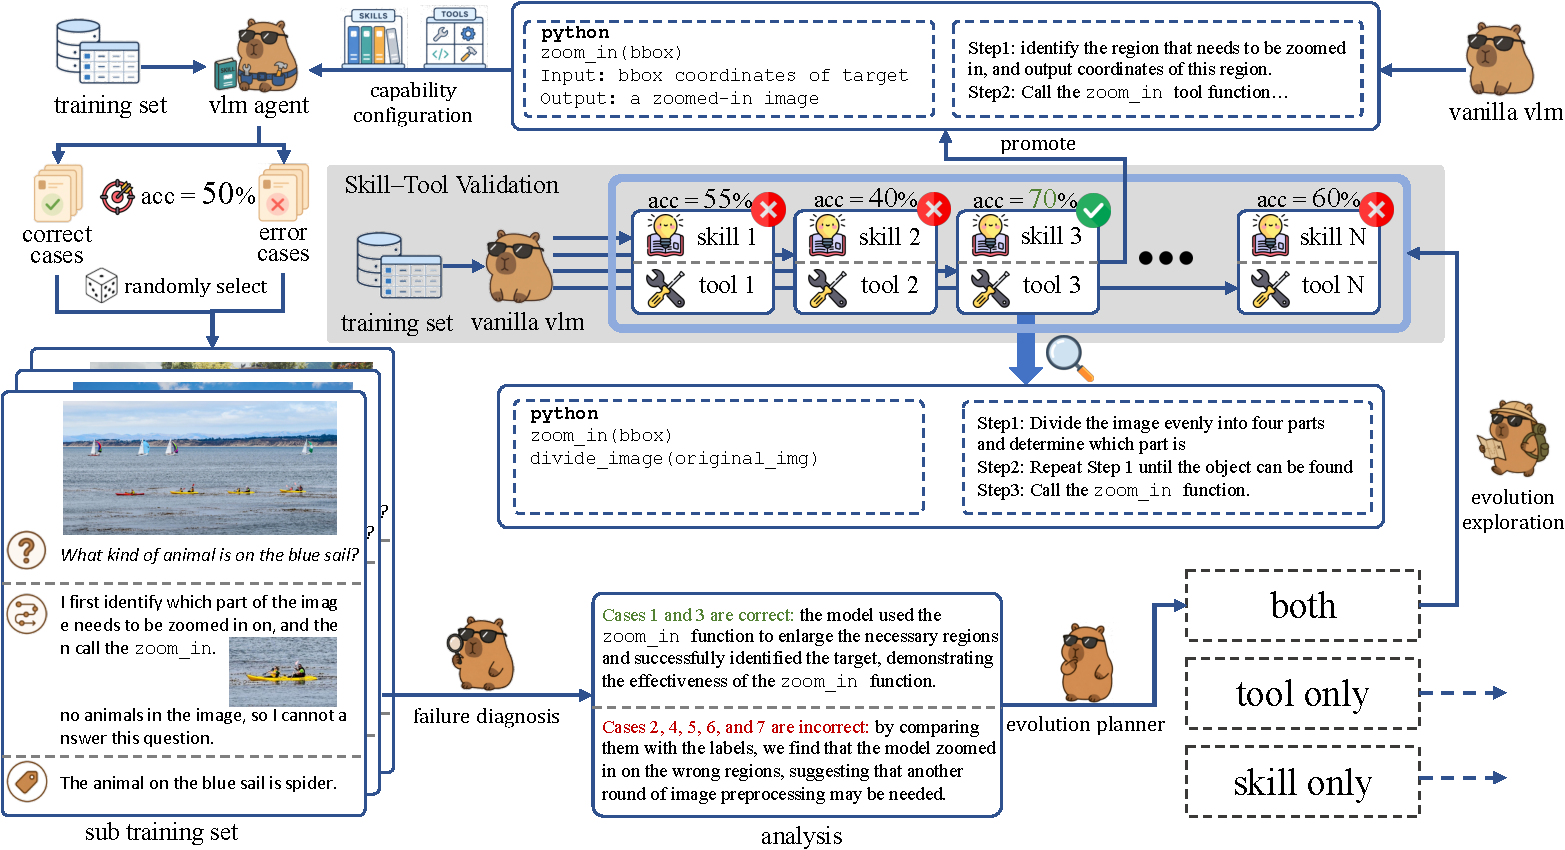
\includegraphics[width=\textwidth]{figures/method.pdf}
  \caption{
    \textbf{\sysname{} evolution loop.}
    On a sampled sub-training set, \sysname{} diagnoses both correct and incorrect attempts,
    explores candidate skill$+$tool capabilities, and promotes the best by validation into a
    persistent library.
  }
  \label{fig:method}
\end{figure*}

\subsection{Problem Formulation}
\label{sec:method_formulation}

Let $\mathcal{D}_{\text{train}} = \{(x_i, y_i, \mathbf{v}_i)\}_{i=1}^{k}$ denote a small training
subset of $k$ cases, where $x_i$ is the question, $y_i$ the ground-truth answer, and $\mathbf{v}_i$
the associated visual input (one or more images).
Let $\pi_\theta$ be a frozen VLM backbone (no gradient updates permitted).
We define a capability set $\mathcal{C} = \{\mathcal{S}, \mathcal{T}\}$, where
$\mathcal{S}$ is a library of \emph{skills} (structured reasoning SOPs) and
$\mathcal{T}$ is a library of \emph{tools} (executable Python programs).
An agent $f_{\mathcal{C}}$ operates by retrieving relevant capabilities from $\mathcal{C}$,
applying them during problem solving, and invoking $\pi_\theta$ for reasoning.
Our goal is to learn $\mathcal{C}$ from $\mathcal{D}_{\text{train}}$ to maximise performance on a
held-out validation set $\mathcal{D}_{\text{val}}$, subject to the constraint
$\nabla_\theta = 0$ (no weight updates).

\subsection{Evolution Loop}
\label{sec:method_loop}

Each evolution iteration over $\mathcal{D}_{\text{train}}$ has three phases
(Figure~\ref{fig:method}).

\textbf{Diagnose.}
The agent solves $\mathcal{D}_{\text{train}}$ with the current $\mathcal{C}$, then samples a
sub-training set $\mathcal{D}_{\text{sub}} \subseteq \mathcal{D}_{\text{train}}$ containing
both correct and incorrect attempts. The \textsc{AnalyzerDecider} inspects
$\mathcal{D}_{\text{sub}}$---the questions, original images $\mathbf{v}_i$, reasoning
traces $\tau_i$, and any intermediate tool outputs---and emits a root-cause analysis grounded
in visual evidence, an identified bottleneck type (\emph{cognitive} when the visual evidence
is available but the reasoning procedure is weak, or \emph{perceptual} when the agent needs a
transformed visual input), and an action $a \in \{\texttt{skill}, \texttt{tool}, \texttt{both}\}$.
Visual input here is essential: deciding whether a crop is misaligned, whether labels are
legible, or whether a processed image introduced artefacts requires inspecting the image, not
just the reasoning trace.

\textbf{Explore.}
Conditioned on the diagnosis, the \textsc{Generator} proposes $M$ candidate skill$+$tool
combinations, each addressing the diagnosed bottleneck with a different strategy or
implementation.

\textbf{Validate and promote.}
Each candidate is evaluated on $\mathcal{D}_{\text{train}}$, and the combination with the
highest accuracy is added to $\mathcal{C}$. Selection by accuracy on
$\mathcal{D}_{\text{train}}$ subsumes both an \emph{origin} requirement (the new capability
must improve over the previous $f_{\mathcal{C}}$ on the cases it targets) and a
\emph{regression} requirement (it must not degrade currently-correct cases). Promoted tools
then go through a mastery phase (Section~\ref{sec:method_tool}) that profiles when each tool
helps before exposing it at inference. The full procedure runs for $N$ iterations (default
$N{=}3$); pseudocode is given in Appendix~\ref{app:impl} (Algorithm~\ref{alg:main}).

\subsection{Skills}
\label{sec:method_skill}

A \emph{skill} is a structured Markdown document with four fields:
\textbf{When-to-Use} (a trigger predicate over question and image type),
\textbf{Strategy} (a numbered step-by-step SOP),
\textbf{Common Pitfalls}, and
\textbf{Worked Example}.
The Generator writes a skill conditioned on the AnalyzerDecider's root-cause analysis; if a
skill covering the same problem class already exists in $\mathcal{S}$, new insights are merged
into it rather than creating a duplicate, preventing library bloat. At inference, the Solver
retrieves the top-$K$ skills by BM25 similarity to the question and appends them to the system
prompt.

\subsection{Tools and Mastery}
\label{sec:method_tool}
\label{sec:method_mastery}

A \emph{tool} is a Python function ($\leq$150 lines) that takes one or more image paths and
returns processed images or extracted data, using standard CV libraries (OpenCV, PIL, NumPy).
The Generator writes a tool conditioned on a perceptual bottleneck diagnosis; representative
examples produced in our experiments include chart re-rendering with enlarged axis labels,
saliency-guided sub-region extraction, and contrast enhancement for low-quality documents.

\paragraph{Mastery profiling.}
For each promoted tool, \sysname{} runs a mastery phase: the tool is applied to a held-out set
of 50 similar cases sampled from $\mathcal{D}_{\text{train}}$, and the agent records per case
whether the tool improved, degraded, or had no effect on the final answer. From this profile,
the agent synthesises a \emph{mastery SOP}---a Markdown document describing the tool's
supported input patterns, negative patterns, and trigger conditions. The mastery SOP is
stored with the tool and consulted at inference to decide whether to invoke it, reducing
false-positive applications that would add latency or visual artefacts. This selective
invocation distinguishes \sysname{} from prior tool-creation
methods~\citep{tang2023creator, cai2024latm} that deploy generated tools indiscriminately.

\subsection{Tool Mastery from External Tool Sets (Mode B)}
\label{sec:method_mastery_ext}

The loop above (\textbf{Mode A}) both \emph{generates} tools and \emph{profiles} their
applicability. When a curated tool set $\mathcal{T}_0 \neq \emptyset$ is already provided,
\sysname{} can operate in \textbf{Mode B}: skip tool generation and apply the mastery
procedure directly to each $t_j \in \mathcal{T}_0$. Skill evolution proceeds unchanged.
Mode B requires no code generation and fewer LLM calls (one mastery profiling pass per tool),
making it practical when tool quality is already high but deployment strategy is unknown.
Experiment~II (Section~\ref{sec:exp2}) evaluates this mode.


\section{Experiments}
% ============================================================
%  §4  Experiments
% ============================================================
\label{sec:experiments}

% ============================================================
\subsection{Experimental Setup}
\label{sec:setup}
% ============================================================

\paragraph{Benchmarks.}
For the evolution-from-scratch setting (Exp~I) we use four visual reasoning benchmarks:
\textbf{ChartQA}~\citep{masry2022chartqa} (multi-step numerical reasoning over charts;
2{,}500 test questions, relaxed accuracy with 5\% tolerance),
\textbf{MathVista}~\citep{lu2023mathvista} (math reasoning grounded in figures and plots;
1{,}000 testmini questions, accuracy),
\textbf{HRBench}~\citep{chen2024hrbench} (perception on $\geq$4K-resolution images;
accuracy), and
\textbf{V$^*$}~\citep{wu2024vstar} (visual search for an object's property;
${\approx}500$ questions, accuracy); the first two stress \emph{cognitive} bottlenecks
while the latter two stress \emph{perceptual} ones.
For the tool-mastery setting (Exp~II) we use \textbf{GTA}~\citep{gta_2024}, a benchmark of
229 real-world tasks with tools across perception, operation, logic, and creativity
categories. GTA reports step-by-step accuracy on tool selection, argument prediction, and
instruction following, plus an end-to-end answer accuracy.
For the RL comparison (Exp~III) we follow the VTool-R1
protocol~\citep{vtoolr1_2025} on its \textbf{Chart} and \textbf{Table} reasoning splits and
reuse \textbf{V$^*$} and \textbf{HRBench4K} as the high-resolution splits of the DeepEyes
protocol~\citep{deepeyes_2025}.

\paragraph{Foundation models.}
Experiment~I evaluates five proprietary and open-weight VLMs:
\textbf{GPT-4o}, \textbf{o4-mini}, \textbf{GPT-5.4}, \textbf{Doubao-Seed-2.0}, and
\textbf{Qwen3.5-27B}.
Experiment~II evaluates \textbf{GPT-4o}, \textbf{GPT-5.4}, and \textbf{Doubao-Seed-2.0}
on the GTA benchmark, plus a controlled \textbf{Doubao-Seed-2.0-Pro} analysis that
inspects how provided-tool skills change with tool abstraction and task environment.
Experiment~III uses the \textbf{Qwen2.5-VL} family (3B, 7B, 32B) to align with the
VTool-R1 evaluation protocol. All VLM weights are \emph{frozen} throughout; no gradient
updates are performed.

\paragraph{Evolution protocol.}
For each benchmark, we sample 20\% of the official training split as
$\mathcal{D}_{\text{train}}$ and run the \sysname{} evolution loop for $N{=}3$ iterations.
The capability set $\mathcal{C}$ is then frozen and evaluated on the held-out
validation / test split. We report the average over three independent random seeds
(different 20\% subsets) to account for sampling variance where repeated runs are
available.

\paragraph{Baselines.}
For Experiment~I, we compare four evolution configurations that isolate the contribution
of each component:
\textbf{None (Base Agent)} invokes the frozen VLM with no evolved capabilities (the
zero-shot baseline);
\textbf{Skill Only} restricts the Generator to producing reasoning skills (no tool
generation);
\textbf{Tool Only} restricts the Generator to producing executable visual tools (no skill
generation);
\textbf{Full} is the unrestricted \sysname{} system, where the AnalyzerDecider chooses on
each case whether to generate a skill, a tool, or both.

\paragraph{Evaluation metrics.}
All primary metrics are task-level accuracy on the held-out split.
For Experiment~II we report four of GTA's five canonical metrics: three
step-by-step metrics---\textbf{InstAcc} (Instruction-Following Accuracy: fraction of
steps executed without errors), \textbf{ToolAcc} (Tool Selection Accuracy), and
\textbf{ArgAcc} (Argument Prediction Accuracy)---and the end-to-end \textbf{AnsAcc}
(Answer Accuracy on full tool-using execution). 
For the supplementary controlled GTA analysis, we also report tool usage rate, average
number of tool calls, and dominant tool-call chains.
Experiment~III follows the VTool-R1 evaluation protocol~\citep{vtoolr1_2025} on Chart
and Table reasoning splits, and uses DeepEyes~\citep{deepeyes_2025} as the RL reference
for high-resolution V$^\star$ and HRBench4K visual-search tasks.

% ============================================================
\subsection{Experiment~I: Autonomous Evolution from Scratch}
\label{sec:exp1}
% ============================================================

We test whether \sysname{} can bootstrap a useful capability library from scratch
($\mathcal{S}{=}\emptyset$, $\mathcal{T}{=}\emptyset$) across five backbones and four
benchmarks, and whether the library remains useful when the query distribution shifts
over time (Section~\ref{sec:method_adaptation}).

\paragraph{Per-benchmark results.}
Table~\ref{tab:evolution_full} reports accuracy for the four configurations on each
backbone. Comparing the Full system to the zero-shot \emph{None} baseline, \sysname{}
improves direct inference on all 20 model--benchmark cells, with an average gain of $+4.7$
accuracy points. The largest gains are on o4-mini / HRBench ($+12.7$), GPT-5.4 / HRBench
($+10.7$), Doubao-Seed-2.0 / V$^*$ ($+8.8$), and Qwen3.5-27B / HRBench ($+8.2$). The
relative strength of \emph{Skill Only} and \emph{Tool Only} also follows the cognitive /
perceptual split: Skill Only is competitive on ChartQA and MathVista, where the gain comes
from better decomposition and calculation procedures, while Tool Only and Full dominate on
HRBench and V$^*$, where sub-region inspection and visual search are central. On a few
cells (GPT-4o / MathVista, Doubao / V$^*$) Skill Only or Tool Only slightly edges out
Full---an expected consequence of leaving capability choice to the AnalyzerDecider rather
than enforcing both per case.

\paragraph{Capability quality.}
Appendix~\ref{app:capability_cases} inspects three representative forms of evolved
capability: a ReFocus-style chart/table editing case, a ZoomEye-style coarse-to-fine
search case, and an interleaved skill that pairs a textual SOP with visual evidence. The
case studies illustrate what \sysname{} generates; they do not claim to reproduce the full
algorithms of ReFocus~\citep{refocus_2025} or ZoomEye~\citep{zoomeye_2024}.

% \iffalse
\begin{table*}[t]
\centering
\small
\setlength{\tabcolsep}{5pt}
\renewcommand{\arraystretch}{1.15}
\begin{tabular}{llcccc}
\toprule
\textbf{Model} & \textbf{Evolution Strategy}
  & \textbf{HRBench}
  & \textbf{MathVista}
  & \textbf{V$^*$}
  & \textbf{ChartQA} \\
\midrule

\multirow{4}{*}{GPT-4o}
  & None (Base Agent)  &0.6386  &0.6711  &0.5828  &0.7552  \\
  & Skill Only         &$0.6733 {\pm} 0.0121$  &$0.7122 {\pm} 0.0038$  &$0.6424 {\pm} 0.0066$  &$0.7785 {\pm} 0.0026$  \\
  & Tool Only          &$0.6452 {\pm} 0.0044$  &$0.6900 {\pm} 0.0029$  &$0.6225 {\pm} 0.0066$  & $0.7722 {\pm} 0.0029$  \\
  & Full               &$0.6886 {\pm} 0.0071$  &$0.7189 {\pm} 0.0029$  &$0.6689 {\pm} 0.0239$  &$0.7799 {\pm} 0.0045$  \\

\midrule

\multirow{4}{*}{o4-mini}
  & None (Base Agent)  &0.73  &0.753333  &0.72847  &0.7833  \\
  & Skill Only         &$0.7724 {\pm} 0.0058$  &$0.7470 {\pm} 0.0107$  &$0.7616 {\pm} 0.0066$  &$0.7866 {\pm} 0.0151$  \\
  & Tool Only          &$0.7457 {\pm} 0.1670$  &$0.7356 {\pm} 0.0328$  &$0.8387 {\pm} 0.0629$  & $0.7920 {\pm} 0.0213$  \\
  & Full               &$0.8571 {\pm} 0.0099$  &$0.7559 {\pm} 0.0055$  &$0.8698 {\pm} 0.0076$  &$0.8007 {\pm} 0.0081$  \\

\midrule

\multirow{4}{*}{gpt5.4}
  & None (Base Agent)  &0.7471  &0.7589  &0.7748  &0.7974  \\
  & Skill Only         &$0.7805 {\pm} 0.0036$  &$0.7752 {\pm} 0.0039$  &$0.7682 {\pm} 0.0199$  &$0.8090 {\pm} 0.0022$  \\
  & Tool Only          &$0.8367 {\pm} 0.0346$  &$0.7663 {\pm} 0.0061$  &$0.8477 {\pm} 0.0132$  & $0.8108 {\pm} 0.0052$  \\
  & Full               &$0.8538 {\pm} 0.0036$  &$0.7815 {\pm} 0.0101$  &$0.8521 {\pm} 0.0233$  &$0.8276 {\pm} 0.0278$  \\

\midrule

\multirow{4}{*}{Doubao-Seed-2.0}
  & None (Base Agent)  &0.8214  &0.8544  &0.8675  &0.8152  \\
  & Skill Only         &$0.8600 {\pm} 0.0049$  &$0.8556{\pm} 0.0109$  &$0.8609 {\pm} 0.0115$  &$0.8198 {\pm} 0.0031$  \\
  & Tool Only          &$0.9005 {\pm} 0.0022$  &$0.8659 {\pm} 0.0061$  &$0.9448 {\pm} 0.0038$  & $0.8156 {\pm} 0.0068$  \\
  & Full               &$0.8990 {\pm} 0.0064$  &$0.8681 {\pm} 0.0105$  &$0.9558 {\pm} 0.0038$  &$0.8347 {\pm} 0.0295$  \\

\midrule

\multirow{4}{*}{Qwen3.5-27B}
  & None (Base Agent)  &0.8171  &0.8088  &0.88079  &0.8114  \\
  & Skill Only         &$0.8721 {\pm} 0.0030$  &$0.8152{\pm} 0.0080$  &$0.8675 {\pm} 0.0066$  &$0.8097 {\pm} 0.0090$  \\
  & Tool Only          &$0.8986 {\pm} 0.0000$  &$0.8241 {\pm} 0.0034$  &$0.9514 {\pm} 0.0101$  & $0.8115 {\pm} 0.0041$  \\
  & Full               &$0.9010 {\pm} 0.0008$  &$0.8252 {\pm} 0.0023$  &$0.9603 {\pm} 0.0175$  &$0.8158 {\pm} 0.0026$  \\

% \midrule

% \multirow{4}{*}{Gemini-3.1-Pro-Preview}
%   & None (Base Agent)  &0.7792  &0.8473  &0.8411  &0.6517  \\
%   & Skill Only         &  &  &  &  \\
%   & Tool Only          &  &  &  &  \\
%   & Full               &  &0.849  &0.8543  &0.7980  \\

\bottomrule
\end{tabular}
\caption{%
  \textbf{Autonomous evolution from scratch.} Accuracy across five VLM backbones and four
  benchmarks. The Full \sysname{} configuration improves over the zero-shot \emph{None}
  baseline on all 20 model--benchmark cells.
}
\label{tab:evolution_full}
\end{table*}

% \begin{table*}[t]
% \centering
% \scriptsize
% \setlength{\tabcolsep}{2.5pt}
% \renewcommand{\arraystretch}{1.12}
% \resizebox{\textwidth}{!}{%
% \begin{tabular}{llcccc}
% \toprule
% \textbf{Model} & \textbf{Evolution Strategy}
%   & \textbf{HRBench}
%   & \textbf{MathVista}
%   & \textbf{V$^*$}
%   & \textbf{ChartQA} \\
% \midrule

% \multirow{4}{*}{GPT-4o}
%   & None (Base Agent)  &$0.6386{\pm}0.014$  &$0.6711{\pm}0.012$  &$0.5828{\pm}0.016$  &$0.7552{\pm}0.011$  \\
%   & Skill Only         &$0.6614{\pm}0.013$  &$0.7077{\pm}0.011$  &$0.6358{\pm}0.015$  &$0.7796{\pm}0.010$  \\
%   & Tool Only          &$0.6414{\pm}0.014$  &$0.6922{\pm}0.012$  &$0.6159{\pm}0.015$  &$0.7693{\pm}0.011$  \\
%   & Full               &$0.6600{\pm}0.013$  &$0.7078{\pm}0.011$  &$0.6423{\pm}0.014$  &$0.7750{\pm}0.010$  \\

% \midrule

% \multirow{4}{*}{o4-mini}
%   & None (Base Agent)  &$0.7300{\pm}0.012$  &$0.7533{\pm}0.010$  &$0.7285{\pm}0.012$  &$0.7833{\pm}0.010$  \\
%   & Skill Only         &$0.7671{\pm}0.011$  &$0.7567{\pm}0.010$  &$0.7550{\pm}0.011$  &$0.7693{\pm}0.011$  \\
%   & Tool Only          &$0.5529{\pm}0.018$  &$0.6978{\pm}0.013$  &$0.7677{\pm}0.011$  &$0.7677{\pm}0.011$  \\
%   & Full               &$0.8457{\pm}0.009$  &$0.7622{\pm}0.010$  &$0.7947{\pm}0.010$  &$0.7917{\pm}0.010$  \\

% \midrule

% \multirow{4}{*}{GPT-5.4}
%   & None (Base Agent)  &$0.7471{\pm}0.012$  &$0.7589{\pm}0.010$  &$0.7748{\pm}0.011$  &$0.7974{\pm}0.010$  \\
%   & Skill Only         &$0.7800{\pm}0.011$  &$0.7711{\pm}0.010$  &$0.7881{\pm}0.010$  &$0.8115{\pm}0.009$ \\
%   & Tool Only          &$0.7971{\pm}0.010$  &$0.7722{\pm}0.010$  &$0.8609{\pm}0.008$  &$0.8161{\pm}0.009$  \\
%   & Full               &$0.8500{\pm}0.009$  &$0.7856{\pm}0.009$  &$0.8742{\pm}0.008$  &$0.8594{\pm}0.008$  \\

% \midrule

% \multirow{4}{*}{Doubao-Seed-2.0}
%   & None (Base Agent)  &$0.8214{\pm}0.010$  &$0.8544{\pm}0.009$  &$0.8675{\pm}0.008$  &$0.8152{\pm}0.009$  \\
%   & Skill Only         &$0.8629{\pm}0.009$  &$0.8433{\pm}0.009$  &$0.8675{\pm}0.008$  &$0.8229{\pm}0.009$ \\
%   & Tool Only          &$0.9000{\pm}0.007$  &$0.8700{\pm}0.008$  &$0.9470{\pm}0.006$  &$0.8078{\pm}0.010$  \\
%   & Full               &$0.9057{\pm}0.007$  &$0.8800{\pm}0.008$  &$0.9536{\pm}0.006$  &$0.8688{\pm}0.008$  \\

% \midrule

% \multirow{4}{*}{Qwen3.5-27B}
%   & None (Base Agent)  &$0.8171{\pm}0.010$  &$0.8088{\pm}0.010$  &$0.8808{\pm}0.008$  &$0.8114{\pm}0.009$  \\
%   & Skill Only         &$0.8192{\pm}0.010$  &$0.8244{\pm}0.009$  &$0.8676{\pm}0.008$  &$0.7994{\pm}0.010$  \\
%   & Tool Only          &$0.8201{\pm}0.010$  &$0.8233{\pm}0.009$  &$0.9603{\pm}0.005$  &$0.8067{\pm}0.009$  \\
%   & Full               &$0.8372{\pm}0.009$  &$0.8222{\pm}0.009$  &$0.9470{\pm}0.006$  &$0.8182{\pm}0.009$  \\

% \bottomrule
% \end{tabular}%
% }
% \caption{%
%   \textbf{Exp~I: Autonomous evolution from scratch.}
%   Accuracy for each evolution strategy across foundation-model blocks and four benchmarks,
%   all starting from an empty capability set.
%   \emph{None} is the zero-shot VLM baseline.
%   \emph{Skill Only} / \emph{Tool Only} ablate one capability type.
%   \emph{Skill~$+$~Tool} is the full \sysname{} system.
%   Standard deviations are temporary layout placeholders and must be replaced with seed-based
%   estimates before submission.
% }
% \label{tab:evolution_full}
% \end{table*}

\paragraph{Online adaptation to distribution shift.}
To simulate real online user traffic---where the task distribution shifts over time as
different users and requests arrive---we replay a non-stationary stream that begins on one
family (HRBench) and then drifts into mixtures dominated by MathVista, ChartQA, and
finally V$^*$. The replay reuses completed per-case outputs, isolating the adaptation
policy from the cost of regenerating capabilities online. We compare \emph{Direct} (no
capabilities), \emph{Static} (capabilities evolved on the initial distribution only and
never updated), \emph{Online adapt} (\sysname{} detects the shift and updates skills and
tools on the new sub-stream), and \emph{Oracle} (capabilities pre-evolved on every family,
an upper bound), each on three stream constructions: \emph{Capability-relevant} (cases
whose outcome depends on the matching capability), \emph{Stress} (cases the matching
capability fixes), and \emph{Natural} (fixed-seed mixture).

Table~\ref{tab:distribution_shift} shows \emph{Online adapt} consistently lands closer to
\emph{Oracle} than to \emph{Static}. On GPT-5.4 capability-relevant it reaches $0.870$
versus $0.636$ static and $0.899$ oracle; on stress, \emph{Direct} collapses to $0.026$,
\emph{Static} reaches $0.391$, and \emph{Online adapt} recovers to $0.947$. On the natural
mix---where many cases do not require a newly-evolved capability---the gain is smaller but
still positive ($0.830$ vs.\ $0.800$ static). The other four backbones follow the same
pattern.

\begin{table}[t]
\centering
\small
\setlength{\tabcolsep}{4pt}
\renewcommand{\arraystretch}{1.12}
\resizebox{\columnwidth}{!}{%
\begin{tabular}{lcccc}
\toprule
\textbf{Replay protocol}
  & \textbf{Direct}
  & \textbf{Static}
  & \textbf{Online adapt}
  & \textbf{Oracle} \\
\midrule
\multicolumn{5}{l}{\emph{GPT-4o (Full)}} \\
Capability-relevant & $0.418{\pm}0.020$ & $0.558{\pm}0.023$ & $0.789{\pm}0.025$ & $0.818{\pm}0.022$ \\
Stress & $0.068{\pm}0.009$ & $0.347{\pm}0.011$ & $0.912{\pm}0.008$ & $0.961{\pm} 0.010$ \\
Natural & $0.664{\pm}0.032$ & $0.673{\pm}0.030$ & $0.702{\pm}0.028$ & $0.705{\pm}0.028$ \\
\midrule
\multicolumn{5}{l}{\emph{o4mini (Full)}} \\
Capability-relevant & $0.467{\pm}0.019$ & $0.626{\pm}0.019$ & $0.852{\pm}0.019$ & $0.881{\pm}0.016$ \\
Stress & $0.047{\pm}0.006$ & $0.412{\pm}0.006$ & $ 0.940{\pm}0.009$ & $0.984{\pm}0.007$ \\
Natural & $0.745{\pm}0.029$ & $0.787{\pm}0.028$ & $0.807{\pm}0.027$ & $0.808{\pm}0.027$ \\
\midrule
\multicolumn{5}{l}{\emph{GPT-5.4 (Full)}} \\
Capability-relevant & $0.479{\pm}0.021$ & $0.636{\pm}0.020$ & $0.870{\pm}0.020$ & $0.899{\pm}0.018$ \\
Stress & $0.026{\pm}0.004$ & $0.391{\pm}0.004$ & $ 0.947{\pm}0.007$ & $0.995{\pm}0.005$ \\
Natural & $0.761{\pm}0.029$ & $0.800{\pm}0.029$ & $0.830{\pm}0.026$ & $0.833{\pm}0.025$ \\
\midrule
\multicolumn{5}{l}{\emph{Qwen3.5-27B (Full)}} \\
Capability-relevant & $0.514{\pm}0.015$ & $0.667{\pm}0.016$ & $ 0.888{\pm}0.020$ & $ 0.917{\pm}0.018$ \\
Stress & $0.122{\pm}0.007$ & $0.488{\pm}0.007$ & $0.940{\pm}0.009$ & $0.984{\pm}0.008$ \\
Natural & $0.821{\pm}0.026$ & $0.847{\pm}0.023$ & $0.861{\pm}0.022$ & $0.862{\pm}0.022$ \\
\midrule
\multicolumn{5}{l}{\emph{Doubao-Seed-2.0 (Full)}} \\
Capability-relevant & $0.635{\pm}0.014$ & $0.773{\pm}0.015$ & $0.900{\pm}0.018$ & $ 0.917{\pm}0.016$ \\
Stress & $0.621{\pm}0.013$ & $0.768{\pm}0.014$ & $0.902{\pm}0.014$ & $0.920{\pm}0.014$ \\
Natural & $0.850{\pm}0.023$ & $0.876{\pm}0.022$ & $0.893{\pm}0.019$ & $0.895{\pm}0.019$ \\
\bottomrule
\end{tabular}%
}
\caption{%
  \textbf{Online adaptation to distribution shift.} Replay accuracy on a non-stationary
  user-traffic stream. \emph{Online adapt} stays close to the \emph{Oracle} upper bound
  and far above \emph{Static} across all five backbones.
}
\label{tab:distribution_shift}
\end{table}

% ============================================================
\subsection{Experiment~II: Learning to Use Pre-Provided Tools}
\label{sec:exp2}
% ============================================================

\paragraph{Results on GTA.}
Table~\ref{tab:gta_detailed} compares \emph{Base Agent} (zero-shot VLM with the provided
GTA tools exposed) to \sysname{} Mode~B (skills $+$ mastery learned on the training set,
no new tool generation) across three backbones. Mode~B improves all three step-level
metrics on every backbone: \textbf{InstAcc}, \textbf{ToolAcc}, and \textbf{ArgAcc} each
gain double-digit points on GPT-5.4 ($+27$, $+33$, $+27$) and Doubao-Seed-2.0 ($+16$,
$+19$, $+16$), and gain $+5$ on GPT-4o. End-to-end \textbf{AnsAcc} also improves on the
two stronger backbones (GPT-5.4 $+2.5$, Doubao $+4.9$). The only regression is GPT-4o
AnsAcc ($-8.2$): the evolved mastery SOP recommends tool invocation in a broader set of
conditions than GPT-4o can reliably execute, leading it to invoke tools on cases it would
have answered correctly without them. This is consistent with the Exp~I observation that
evolution gains depend on the backbone's instruction-following capacity.

\begin{table}[t]
\centering
\small
\setlength{\tabcolsep}{4pt}
\renewcommand{\arraystretch}{1.15}
\resizebox{\columnwidth}{!}{%
\begin{tabular}{llcccc}
\toprule
\textbf{Model} & \textbf{Method}
  & \textbf{ToolAcc}
  & \textbf{ArgAcc}
  & \textbf{InstAcc}
  & \textbf{AnsAcc} \\
\midrule

\multirow{2}{*}{GPT-4o}
  & Base Agent             & 80.3 & 62.0 & 52.0 & 66.1 \\
  & Skill Evolution (Ours) & 85.3 & 67.4 & 57.3 & 57.9 \\

\midrule

\multirow{2}{*}{GPT-5.4}
  & Base Agent             & 53.0 & 36.9 & 33.3 &  66.1 \\
  & Skill Evolution (Ours) & 85.7 & 63.4 & 59.9 & 68.6 \\

\midrule

\multirow{2}{*}{Doubao-Seed-2.0}
  & Base Agent             & 67.7 & 45.5 & 41.6 & 76.9 \\
  & Skill Evolution (Ours) & 86.4 & 61.3 & 57.7 & 81.8 \\

\bottomrule
\end{tabular}%
}
\caption{%
  \textbf{Learning to use pre-provided tools on GTA.}
  \sysname{} Mode~B (skills $+$ mastery only; no new tool generation) improves all
  step-level metrics on every backbone, and improves end-to-end answer accuracy on the
  two stronger backbones.
}
\label{tab:gta_detailed}
\end{table}

\paragraph{Controlled tool-policy analysis.}
Table~\ref{tab:gta_controlled} runs a complementary controlled study on GTA with
Doubao-Seed-2.0-Pro to inspect what the learned policy actually does when either the tool
abstraction or the task environment changes. Two findings stand out. First, fixing the
environment to OCR$+$Calculator, stronger composite tools compress the policy: atomic
tools reach $86.7$ via an \texttt{OCR}$\to$\texttt{Calculator} chain ($22/30$ cases),
while \texttt{VisualArithmeticSolver} reaches $90.0$ with a one-call policy ($30/30$).
Second, the same \texttt{OCR} tool plays different roles in different environments: in
OCR$+$Calc it feeds arithmetic (\texttt{OCR}$\to$\texttt{Calculator}, $19/20$), while in
OCR$+$Search it feeds external lookup
(\texttt{OCR}$\to$\texttt{Search}$\to$\texttt{OCR}$\to$\texttt{Search}, $20/20$).

\begin{table}[t]
\centering
\small
\setlength{\tabcolsep}{4pt}
\renewcommand{\arraystretch}{1.15}
\resizebox{\columnwidth}{!}{%
\begin{tabular}{llcccc}
\toprule
\textbf{Study} & \textbf{Condition} & \textbf{Cases} & \textbf{Acc.}
& \textbf{Tool use} & \textbf{Avg. calls} \\
\midrule
Tool strength & Direct, no tools & 30 & 83.3 & 0.0 & 0.00 \\
Tool strength & Atomic OCR+Calc & 30 & 86.7 & 100.0 & 1.83 \\
Tool strength & Composite VAS & 30 & 90.0 & 100.0 & 1.00 \\
\midrule
OCR role & OCR+Calc env & 20 & 80.0 & 100.0 & 2.20 \\
OCR role & OCR+Search env & 20 & 85.0 & 100.0 & 2.35 \\
\bottomrule
\end{tabular}%
}
\caption{%
  \textbf{Controlled tool-policy analysis on GTA (Doubao-Seed-2.0-Pro).}
  Top: stronger composite tools compress the policy at higher accuracy. Bottom: the same
  \texttt{OCR} tool exhibits different downstream behavior in different environments
  (dominant call chains discussed in prose). Acc./Tool use in \%; Avg. calls is a count.
}
\label{tab:gta_controlled}
\end{table}


% TODO: Insert MIRA subset results when available.

% ============================================================
\subsection{Experiment~III: RL and Self-Evolution Across Visual Tool Tasks}
\label{sec:exp3}
% ============================================================

We compare \sysname{} against task-specific RL on three task families using the
Qwen2.5-VL family (3B, 7B, 32B): Chart and Table reasoning under the VTool-R1
protocol~\citep{vtoolr1_2025}, and high-resolution V$^\star$ and HRBench4K under the
DeepEyes protocol~\citep{deepeyes_2025}. Two cells (32B \sysname{}\,$+$\,RL on Chart and
Table) are runs not yet completed.

\paragraph{Chart and Table reasoning.}
Using the gap-recovery fraction $(\sysname{}-\text{Direct})/(\text{RL}-\text{Direct})$,
\sysname{} recovers $65.7\%$ and $99.4\%$ of the Chart gap at 3B and 7B respectively, and
\emph{exceeds} RL at 32B ($86.4$ vs.\ $84.3$). On Table, recovery is
$67.5\%$ / $91.4\%$ / $46.8\%$. \sysname{}\,$+$\,RL further beats RL alone by $1$--$3$
points wherever the row is reported, indicating that the two interventions compose
additively.

\paragraph{High-resolution visual search.}
On V$^\star$ and HRBench4K, \sysname{} alone matches or beats task-specific RL at every
scale: it gains $+6.3$ / $+1.0$ / $\pm 0.0$ over RL on V$^\star$ (3B / 7B / 32B) and
$+4.0$ / $+0.7$ / $+5.1$ on HRBench4K. Adding \sysname{} on top of the RL-trained
policy raises 7B V$^\star$ to $92.7$ and 7B HRBench4K to $81.3$, the strongest
configurations in those cells.

\paragraph{Cost.}
\sysname{} performs no weight updates: an evolution run uses 20\% of each benchmark's
training split for $N{=}3$ passes and invokes the frozen VLM for solving, diagnosis,
generation, and validation. The comparison therefore shows that across these three task
families, \sysname{} recovers most of the RL gain on Chart/Table and matches or beats
RL on high-resolution visual search, while composing additively with RL when both are
available.
\begin{table}[t]
\centering
\scriptsize
\setlength{\tabcolsep}{4pt}
\renewcommand{\arraystretch}{1.14}
\resizebox{\columnwidth}{!}{%
\begin{tabular}{llcccc}
\toprule
\textbf{Backbone} & \textbf{Variant}
  & \textbf{Chart} & \textbf{Table}
  & \textbf{V$^\star$} & \textbf{HRBench4K} \\
\midrule
\multirow{4}{*}{Qwen2.5-VL-3B}
  & Direct              & 45.3995 & 43.0921 & 71.20 & 63.62 \\
  & RL                  & 66.95    & 56.25    &78.01  &66.50  \\
  & \sysname{}          & 59.56   & 51.97   & 84.29 & 70.50 \\
  & \sysname{} + RL     & 68.28   & 59.54   &85.34  &71.25  \\
\midrule
\multirow{4}{*}{Qwen2.5-VL-7B}
  & Direct              & 56.0532 & 56.9078 & 79.06 & 70.50 \\
  & RL                  & 75.18   & 68.42   &84.82  &74.38  \\
  & \sysname{}          & 75.060  & 67.43   & 85.86 &75.12 \\
  & \sysname{} + RL     & 76.88   & 69.41   &92.67   &81.25  \\
\midrule
\multirow{4}{*}{Qwen2.5-VL-32B}
  & Direct              & 81.3559 & 82.8947 & 81.68 & 75.62 \\
  & RL                  & 84.3    & 84.3    &88.48  &72.88  \\
  & \sysname{}          & 86.44    & 83.55   & 88.48   & 78.00 \\
  & \sysname{} + RL     &     &    &91.10    &76.38  \\
\bottomrule
\end{tabular}%
}
\caption{%
  \textbf{Self-evolution vs.\ task-specific RL across three task families.}
  Accuracy (\%). \sysname{} alone matches or beats RL on all six high-resolution cells
  and recovers most of the Chart/Table gap; \sysname{}\,$+$\,RL is additive in nearly
  every cell. Blank cells are runs not yet completed.
}
\label{tab:rl_combined}
\end{table}
% \begin{table*}[t]
% \centering
% \scriptsize
% \setlength{\tabcolsep}{4pt}
% \renewcommand{\arraystretch}{1.14}
% \begin{tabular}{llcccc}
% \toprule
% \textbf{Backbone} & \textbf{Variant}
%   & \textbf{Chart} & \textbf{Table}
%   & \textbf{V$^\star$} & \textbf{HRBench4K} \\
% \midrule
% \multirow{4}{*}{Qwen2.5-VL-3B}
%   & Direct              & 45.3995 & 43.0921 & 56.6 & 47.4 \\
%   & RL                  & 64.0    & 57.9    & 82.8 & 70.1 \\
%   & \sysname{}          & 59.56   & 51.97   & 81.1 & 70.0 \\
%   & \sysname{} + RL     & 68.28   & 59.54   & 83.3 & 71.1 \\
% \midrule
% \multirow{4}{*}{Qwen2.5-VL-7B}
%   & Direct              & 56.0532 & 56.9078 & 71.2 & 68.8 \\
%   & RL                  & 75.18   & 68.09   & 88.8 & 73.1 \\
%   & \sysname{}          & 75.060  & 67.43   & 85.8 & 75.3 \\
%   & \sysname{} + RL     & 76.88   & 69.41   & 91.1  & 77.7 \\
% \midrule
% \multirow{4}{*}{Qwen2.5-VL-32B}
%   & Direct              & 81.3559 & 82.8947 & 87.9 & 73.9 \\
%   & RL                  & 84.3    & 84.3    & 93.3 & 75.2 \\
%   & \sysname{}          & 84.2    & 83.55   & 93.2   & 75.1 \\
%   & \sysname{} + RL     & 85.5    & 84.9    &    &  \\
% \bottomrule
% \end{tabular}
% \caption{%
%   \textbf{Exp~III: unified comparison of direct inference, RL, self-evolution, and
%   self-evolution+RL.}
%   Scores are accuracy (\%). Chart and Table entries follow the VTool-R1 protocol; their RL rows
%   are VTool-R1 GRPO results and their \sysname{}+RL rows add the self-evolved capability on top
%   of the RL-trained policy. V$^\star$ and HRBench4K entries follow the DeepEyes high-resolution
%   evaluation; their RL rows are DeepEyes results where reported. A dash means the corresponding
%   same-backbone or combined run is not reported in the source table and is not inferred here.
% }
% \label{tab:rl_combined}
% \end{table*}

% TODO: Insert combined skill+RL results when available.

% ============================================================
\subsection{Ablation Studies}
\label{sec:ablation}
% ============================================================

The \emph{Skill Only} and \emph{Tool Only} rows of Table~\ref{tab:evolution_full} already isolate
the contribution of each capability type, so we use the remaining ablation budget to study the
\emph{mechanisms} that drive those gains rather than rerunning the same capability-type
comparison. Specifically, we ask whether the improvement comes from (i) failure-specific
capability generation as opposed to generic prompting, (ii) multimodal failure diagnosis as
opposed to text-only reflection, (iii) mastery-gated tool exposure as opposed to unconditional
deployment, and (iv) persistent cross-case capability reuse as opposed to per-case retry. The
full mechanism table, per-ablation discussion, and sensitivity curves are deferred to
Appendix~\ref{app:ablation_mechanisms} for space.


\section{Discussion}
% ============================================================
%  §5  Discussion
% ============================================================
\label{sec:discussion}

\paragraph{When does evolution help?}
The results suggest a practical diagnostic rather than a universal taxonomy. If failures can be
fixed by changing the procedure the agent follows, skill evolution is the lower-cost first
choice. If the agent needs a different view of the image before the evidence is accessible,
tool evolution becomes necessary. A practitioner targeting a new benchmark can use a small pilot
run ($k{\approx}25$, $N{=}1$) to inspect which kinds of capabilities are generated and whether
they transfer beyond the triggering examples.

\paragraph{Limitations.}
Several limitations bound the scope of our conclusions.
\textit{(a) Short evolution horizon.}
We report results at $N{=}3$ iterations; the evolution dynamics suggest gains plateau
around $N{=}5$, but we have not evaluated whether longer runs (e.g.\ $N{>}10$) eventually
overfit the training distribution.
\textit{(b) Tool quality ceiling.}
Tool effectiveness is bounded by the VLM's Python coding ability.
For benchmarks requiring specialised computer vision operations beyond standard libraries
(e.g.\ learned feature extractors), the Generator may fail to produce valid tools, limiting
the perceptual gains.
\textit{(c) Benchmark scope.}
We evaluate on four main visual reasoning benchmarks plus GTA and VTool-R1-aligned splits.
Broader coverage across additional domains (e.g.\ video QA, 3D spatial reasoning, medical
imaging) is needed before making stronger claims about the generality of the proposed
cognitive/perceptual decision rule.
\textit{(d) API cost.}
Each training case incurs up to $\sim$15K tokens (attempt + failure analysis + generation +
validation), summing to $\sim$3M tokens per benchmark run.  While negligible compared to RL
training, this cost should be accounted for when comparing training-free methods.

\paragraph{Future directions.}
Three extensions merit investigation.
First, \emph{cross-benchmark skill transfer}: skills generated from ChartQA failures may
transfer to MathVista (both involve structured data reading); a shared skill library across
benchmarks could reduce per-benchmark cold-start cost.
Second, \emph{image generation as a reasoning tool}: rather than only processing existing images,
the agent could generate hypothetical visualisations (e.g.\ mentally redrawing a chart in a
clearer format) using image generation APIs, extending the ``think with images'' paradigm
\citep{vtoolr1_2025} to internally imagined percepts.
Third, \emph{online evolution}: rather than a fixed pre-deployment training phase, the agent
could evolve capabilities during deployment, adapting to the distribution shift of live queries.


\section{Conclusion}
% ============================================================
%  §  Conclusion
% ============================================================
\label{sec:conclusion}

\sysname{} is a training-free framework in which a frozen VLM agent evolves a
task-family-specific library of reasoning skills and executable visual tools from a small
labeled training subset, with the Analyzer choosing on each case whether
to emit a skill, a tool, or both. A mastery skill paired with each generated tool gates
its invocation at inference, and an online adaptation loop refreshes the library when the
query distribution shifts.

Across four visual-reasoning benchmarks and five backbones, \sysname{} improves direct
inference on all 20 model--benchmark cells; on GTA it lifts every step-level tool-use
metric across all tested backbones; and against task-specific RL (VTool-R1, DeepEyes),
\sysname{} matches or beats RL on high-resolution perception, recovers most of the
structured-VQA gap, and composes additively with RL when both are available. These
results suggest a substantial part of task-specific VLM adaptation can be obtained
without gradient updates, by letting the agent shape its capability library.


% ---- Bibliography ----
\bibliography{references}

% ---- Appendix ----
\appendix
\clearpage
% ============================================================
%  Appendix
% ============================================================

\section{Implementation Details}
\label{app:impl}

\paragraph{Algorithm.}
Algorithm~\ref{alg:main} gives the full \sysname{} evolution procedure described in
Section~\ref{sec:method_loop}.

\begin{algorithm}[h]
\SetAlgoLined
\KwIn{$\mathcal{D}_{\text{train}}$, frozen VLM $\pi_\theta$, iterations $N$, candidates $M$}
\KwOut{Capability set $\mathcal{C} = (\mathcal{S}, \mathcal{T})$}
$\mathcal{C} \leftarrow (\emptyset, \emptyset)$\;
\For{$n = 1$ \KwTo $N$}{
  Solve $\mathcal{D}_{\text{train}}$ with $f_{\mathcal{C}}$; collect attempts\;
  $\mathcal{D}_{\text{sub}} \leftarrow$ sample from $\mathcal{D}_{\text{train}}$\;
  $a, r \leftarrow \textsc{AnalyzerDecider}(\mathcal{D}_{\text{sub}};\, \pi_\theta)$\;
  $\{(s_m, t_m)\}_{m=1}^{M} \leftarrow \textsc{Generator}(a, r;\, \pi_\theta)$\tcp*{$s_m$ paired with $t_m$ acts as its mastery SOP}
  $m^\star \leftarrow \arg\max_{m} \mathrm{Acc}\bigl(f_{\mathcal{C} \cup (s_m, t_m)};\, \mathcal{D}_{\text{train}}\bigr)$\;
  \If{accuracy improves}{
    $\mathcal{C} \leftarrow \mathcal{C} \cup \{(s_{m^\star}, t_{m^\star})\}$\;
  }
}
\Return{$\mathcal{C}$}\;
\caption{\sysname{} evolution loop.}
\label{alg:main}
\end{algorithm}

\paragraph{Role prompts.}
\sysname{} uses three role-specific system prompts for the same base VLM:
\textit{Solver} (standard QA prompt with capability context injected),
\textit{AnalyzerDecider} (root-cause analysis and decision), and
\textit{Generator} (skill or tool generation).
All prompts are provided in full at \url{[anonymised repository]}.

\paragraph{Skill retrieval.}
At inference time, the Solver retrieves the top-$K{=}3$ skills from $\mathcal{S}$ using BM25
cosine similarity over skill titles and When-to-Use fields.
Retrieved skill text is appended to the system prompt.

\paragraph{Tool invocation.}
The Solver inspects each tool's mastery SOP to decide whether to invoke it on the current input.
If the input matches a tool's supported patterns, the tool is applied and its output image(s)
are appended to the multimodal context.
Tool execution is sandboxed with a 30-second timeout and resource limits.

\paragraph{Hyperparameters.}
Table~\ref{tab:hyperparams} lists all hyperparameter settings.

\begin{table}[h]
\centering
\footnotesize
\setlength{\tabcolsep}{3pt}
\caption{Hyperparameter settings.}
\label{tab:hyperparams}
\begin{tabular}{@{}>{\raggedright\arraybackslash}p{0.28\columnwidth}
                >{\raggedright\arraybackslash}p{0.16\columnwidth}
                >{\raggedright\arraybackslash}p{0.44\columnwidth}@{}}
\toprule
\textbf{Parameter} & \textbf{Value} & \textbf{Description} \\
\midrule
$k$         & 200        & Training cases per benchmark \\
$N$         & 3          & Evolution iterations \\
$K$         & 3          & Skills retrieved per query \\
Max tool lines & 150     & Max lines for generated Python tool \\
Mastery sample & 50      & Cases for mastery profiling \\
Regression buffer & 20   & Cases for tool regression test \\
Temperature & 0.7        & Generator temperature \\
Max tokens (gen.) & 2048 & Max tokens for capability generation \\
\bottomrule
\end{tabular}
\end{table}

\paragraph{Compute.}
Experiments use the frozen VLM backbones listed in Section~\ref{sec:setup}.
Total API calls per benchmark: $\leq k \times N \times 3 = 1{,}800$ calls
(solver + analyzer + generator, upper bound).
Estimated token usage: $\sim$3M tokens per benchmark.
No GPU training is performed.

\section{Mechanism Ablations}
\label{app:ablation_mechanisms}

Experiment~I in the main paper already isolates the contribution of each capability
\emph{type}: the \emph{None}, \emph{Skill Only}, \emph{Tool Only}, and \emph{Full} rows of
Table~\ref{tab:evolution_full} answer whether skills, tools, or both account for the
observed gains. The ablations here test a complementary question: when the Full system is
used, which \emph{mechanisms} inside the evolution loop (Section~\ref{sec:method_loop}) are
doing the work? Each variant removes one design decision and holds the rest fixed, so each
row of Table~\ref{tab:ablation_mechanism} rules out one alternative explanation for the
Full system's gains.

\paragraph{Setup.}
All variants use the same protocol as Experiment~I (frozen GPT-5.4 backbone; 20\% of each
benchmark's training split as $\mathcal{D}_{\text{train}}$; $N{=}3$ evolution iterations;
$M$ candidate skill$+$tool combinations per iteration) and rebuild $\mathcal{C}$ from
scratch so any deficit reflects the ablated mechanism rather than a carried-over artifact.
The two primary benchmarks are \textbf{ChartQA} (cognitive / procedural) and
\textbf{HRBench} (perceptual / high-resolution); \textbf{MathVista} and \textbf{V$^\star$}
are reported as secondary checks.

\paragraph{Main mechanism table.}
Table~\ref{tab:ablation_mechanism} reports six ablation variants spanning the four
mechanism families: diagnosis (whether the AnalyzerDecider sees correct cases and visual
input), exploration (multi-candidate generation), inference-time gating (paired mastery
skill), and persistence (cross-case library). The Full row reproduces the Full entry from
Table~\ref{tab:evolution_full} for reference.

\begin{table*}[t]
\centering
\small
\setlength{\tabcolsep}{4pt}
\renewcommand{\arraystretch}{1.18}
\begin{tabular}{lp{0.34\textwidth}cccc}
\toprule
\textbf{Variant} & \textbf{Ablated mechanism}
  & \textbf{ChartQA} & \textbf{HRBench}
  & \textbf{MathVista} & \textbf{V$^\star$} \\
\midrule
Full \sysname{}              & --- (full evolution loop)
  & & & & \\
\midrule
Generic Skill                & evolved library $\to$ hand-neutral task prompt
  & & & & \\
Failure-Only Diagnosis       & AnalyzerDecider sees only incorrect cases
  & & & & \\
Text-only Diagnosis          & AnalyzerDecider sees no images or tool artefacts
  & & & & \\
Single-Candidate ($M{=}1$)   & one Generator proposal per iteration; no selection
  & & & & \\
No Paired Mastery Skill      & tool emitted without its paired skill (action $=$ both)
  & & & & \\
No Persistence               & capabilities not stored across cases
  & & & & \\
\bottomrule
\end{tabular}
\caption{%
  \textbf{Mechanism ablations.}
  Each row removes one mechanism from \sysname{} while holding the rest fixed
  (GPT-5.4; 20\% training split; $N{=}3$). The Full row reproduces the Full entry from
  Table~\ref{tab:evolution_full}. Numbers will be filled in once the corresponding runs
  complete.
}
\label{tab:ablation_mechanism}
\end{table*}

\subsection{Generic Skill vs. Evolved Capability}
\label{app:abl_generic}

\paragraph{What is removed.}
The evolved capability library is replaced with a single hand-neutral task prompt that
gives generic task advice (for ChartQA: ``read the chart carefully, identify relevant
values, reason step by step''; for HRBench: ``inspect local details before answering and
verify the target object''). No diagnosis, generation, validation, or persistence is run.

\paragraph{What this rules out.}
A pure prompt-engineering account would predict that Generic Skill closes most of the gap
to Full, since the evolved skills are themselves natural-language SOPs. If Generic Skill
improves over Direct by only a small margin and stays well below Full, the gap is
attributable to mechanism-level evolution---failure-specific procedures, applicability
triggers, and pitfalls that a generic prompt cannot anticipate---rather than to the
presence of any task-aware prompt.

\subsection{Failure-Only Diagnosis}
\label{app:abl_failure_only}

\paragraph{What is removed.}
The AnalyzerDecider only sees the incorrect cases in the sampled sub-training set; the
correct cases are dropped. Everything else---multimodal input, multi-candidate
exploration, paired mastery skill, persistence---is unchanged.

\paragraph{What this rules out.}
Most prior self-improvement work treats correct cases as nothing to learn from. This
variant tests that assumption directly. If Failure-Only Diagnosis matches Full, then the
correct cases carry no useful diagnostic signal and the abstract's framing of ``diagnoses
both correct and incorrect attempts'' is decorative. A gap supports the design choice:
correct attempts tell the AnalyzerDecider \emph{which sub-patterns the current
$\mathcal{C}$ already handles}, which sharpens the next capability proposal toward what is
still missing.

\subsection{Text-only Diagnosis}
\label{app:abl_textonly}

\paragraph{What is removed.}
The AnalyzerDecider's inputs are restricted to text only: the question, the agent's answer
(correct or incorrect), the ground-truth answer, and the reasoning trace. No original
image, no intermediate tool output, and no processed visual artefact is passed in.

\paragraph{What this rules out.}
Text reflection can say \emph{that} an answer was wrong, but it cannot tell whether a
crop was misaligned, whether a zoomed region missed the target, or whether a processed
image introduced artefacts. We expect the gap to Full to be largest on the perceptual
benchmarks (HRBench, V$^\star$). On ChartQA the gap should be smaller because many
failures there are procedural; a small ChartQA gap with a large HRBench/V$^\star$ gap is
itself the signature of the visual-diagnosis claim.

\subsection{Single-Candidate ($M{=}1$)}
\label{app:abl_single_candidate}

\paragraph{What is removed.}
The Generator produces a single capability proposal per iteration (the same setting as
typical generate-then-validate tool-creation methods such as
CREATOR~\citep{DBLP:conf/emnlp/QianH0Q0J23} and LATM~\citep{DBLP:conf/iclr/Cai00CZ24}). The validate-and-promote
step (Eq.~\ref{eq:selection}) collapses to a binary accept/reject of that single
candidate against the training set.

\paragraph{What this rules out.}
A reviewer might ask whether the multi-candidate $\arg\max$ in Eq.~\ref{eq:selection} is
load-bearing or whether the first proposal is usually good enough. If Single-Candidate
roughly matches Full, the exploration step is decorative. A measurable gap shows that
diverse candidates plus selection by training-set accuracy is what turns a noisy proposal
distribution into a reliably improving library.

\subsection{No Paired Mastery Skill}
\label{app:abl_mastery}

\paragraph{What is removed.}
When the AnalyzerDecider's action is \texttt{both}, the Generator emits only the tool and
not its paired mastery skill. The tool is added to $\mathcal{T}$ but has no
$\textsc{When-to-Use}$ predicate gating its invocation at inference, so any skill
retrieval that surfaces a tool reference exposes the tool unconditionally.

\paragraph{What this rules out.}
Prior tool-creation methods deploy generated tools indiscriminately. The paired-skill
design in Section~\ref{sec:method_mastery} predicts that gating tool invocation by
retrieval of an applicability-encoding skill is what keeps tool usage selective.
No Paired Mastery Skill is expected to keep or even increase tool-usage rate but reduce
accuracy on benchmarks where naive tool exposure can hurt---MathVista is the canonical
cautionary case.

\subsection{No Persistence}
\label{app:abl_persistence}

\paragraph{What is removed.}
Capabilities promoted during one iteration are not stored in $\mathcal{C}$. The agent can
still reflect on a case and immediately retry it with the generated capability, but the
capability is discarded before the next case is processed, so no cross-case retrieval
occurs.

\paragraph{What this rules out.}
A retry-only account would predict that most of Full's gain comes from in-place retry on
the triggering case rather than from cross-case reuse. If No Persistence matches Full on
held-out accuracy, the library is a bookkeeping device with no inferential value. A gap
shows that the system's advantage comes from accumulating capabilities that future cases
can retrieve, not just from one more attempt at the triggering case. ChartQA is the
cleanest test because failures there form recurring families (stacked-bar boundary
reading, multi-series selection) that a single capability can fix across many held-out
cases.

\subsection{Sensitivity to Training Subset Size and Iteration Count}
\label{app:abl_sensitivity}

The main paper fixes the training subset at 20\% of each benchmark's training split and
runs $N{=}3$ evolution iterations. A sensitivity sweep over smaller fractions (e.g.\ 5\%,
10\%) and over $N \in \{1, 3, 5\}$ tests how quickly the library saturates: a small subset
should already expose the most frequent procedural / perceptual patterns, with diminishing
returns as the subset grows; $N{=}1$ should miss capabilities that only surface after
earlier ones reshape the trajectory, while $N{=}3$ and $N{=}5$ should produce comparable
libraries. We treat this as a robustness check rather than a tuning study; the operating
point is chosen to fit the per-benchmark budget.

\subsection{Summary}
\label{app:abl_summary}

Read together, the six mechanism ablations are designed to triangulate the same claim
from six different angles. Generic Skill rules out a pure prompt-engineering explanation;
Failure-Only Diagnosis rules out ``correct cases carry no signal''; Text-only Diagnosis
rules out ``text reflection is enough'' and supports the visual-diagnosis channel;
Single-Candidate rules out ``the first proposal is good enough'' and supports
multi-candidate exploration; No Paired Mastery Skill rules out ``expose every generated
tool'' and supports applicability-bounded deployment; and No Persistence rules out
``per-case retry is enough'' and supports cross-case capability accumulation. The
expected pattern is that removing any one mechanism reduces held-out accuracy noticeably,
but no single ablation collapses the system---consistent with the design view that the
six mechanisms implement complementary aspects of capability evolution rather than
redundant copies of the same underlying lever.

\paragraph{Practical diagnostic.}
The mechanism ablations also suggest a practical rule of thumb for new task families. If
the bottleneck is procedural---visual evidence is present but the reasoning is weak---skill
evolution is the lower-cost first choice; if a different view of the image is required
before the evidence becomes accessible, tool evolution is necessary. A practitioner
targeting a new benchmark can use a small pilot run (e.g.\ 5\% of the training split with
$N{=}1$) to inspect which kinds of capabilities are generated and whether they transfer
beyond the triggering examples.

\section{Additional Results}
\label{app:results}

\subsection{Training Set Size Sensitivity}

\begin{figure}[ht]
\centering
\fbox{\rule{0pt}{3cm}\rule{0.7\columnwidth}{0pt}}
\caption{Placeholder for ChartQA accuracy vs.\ training set size
$k \in \{10, 25, 50, 100, 200\}$ at $N{=}3$ iterations.}
\label{fig:k_sensitivity}
\end{figure}

Figure~\ref{fig:k_sensitivity} shows ChartQA accuracy as a function of training set size
$k \in \{10, 25, 50, 100, 200\}$ at $N{=}3$ iterations.

\subsection{Per-Category Analysis on ChartQA}

% TODO: Insert breakdown of accuracy gains by chart type (bar, line, pie, scatter).

\subsection{Distribution-Shift Adaptation: Time Series and Aggregates}
\label{app:distribution_shift_timeseries}

Figure~\ref{fig:distribution_shift} in the main paper aggregates the distribution-shift
experiment across backbones and stream constructions. This appendix shows the per-step
trajectory along the stream (Figure~\ref{fig:distribution_shift_timeseries}) and the
full per-backbone numerical aggregates (Table~\ref{tab:distribution_shift}).

\begin{figure}[ht]
  \centering
  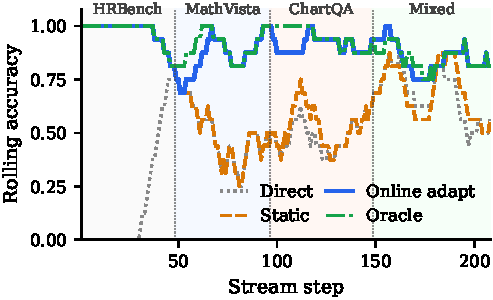
\includegraphics[width=\columnwidth]{figures/distribution_shift_timeseries.pdf}
  \caption{%
    \textbf{Rolling accuracy along the natural stream (GPT-5.4).}
    Phase labels above the plot mark the newly introduced family at each shift; earlier
    families remain present in the mix. \emph{Static} lags at each shift; \emph{Online
    adapt} catches up to \emph{Oracle} within a 2--7 case detection latency.
  }
  \label{fig:distribution_shift_timeseries}
\end{figure}

\begin{table}[ht]
\centering
\small
\setlength{\tabcolsep}{4pt}
\renewcommand{\arraystretch}{1.12}
\resizebox{\columnwidth}{!}{%
\begin{tabular}{lcccc}
\toprule
\textbf{Replay protocol}
  & \textbf{Direct}
  & \textbf{Static}
  & \textbf{Online adapt}
  & \textbf{Oracle} \\
\midrule
\multicolumn{5}{l}{\emph{GPT-4o (Full)}} \\
Capability-relevant & $0.418{\pm}0.020$ & $0.558{\pm}0.023$ & $0.789{\pm}0.025$ & $0.818{\pm}0.022$ \\
Stress & $0.068{\pm}0.009$ & $0.347{\pm}0.011$ & $0.912{\pm}0.008$ & $0.961{\pm} 0.010$ \\
Natural & $0.664{\pm}0.032$ & $0.673{\pm}0.030$ & $0.702{\pm}0.028$ & $0.705{\pm}0.028$ \\
\midrule
\multicolumn{5}{l}{\emph{o4mini (Full)}} \\
Capability-relevant & $0.467{\pm}0.019$ & $0.626{\pm}0.019$ & $0.852{\pm}0.019$ & $0.881{\pm}0.016$ \\
Stress & $0.047{\pm}0.006$ & $0.412{\pm}0.006$ & $ 0.940{\pm}0.009$ & $0.984{\pm}0.007$ \\
Natural & $0.745{\pm}0.029$ & $0.787{\pm}0.028$ & $0.807{\pm}0.027$ & $0.808{\pm}0.027$ \\
\midrule
\multicolumn{5}{l}{\emph{GPT-5.4 (Full)}} \\
Capability-relevant & $0.479{\pm}0.021$ & $0.636{\pm}0.020$ & $0.870{\pm}0.020$ & $0.899{\pm}0.018$ \\
Stress & $0.026{\pm}0.004$ & $0.391{\pm}0.004$ & $ 0.947{\pm}0.007$ & $0.995{\pm}0.005$ \\
Natural & $0.761{\pm}0.029$ & $0.800{\pm}0.029$ & $0.830{\pm}0.026$ & $0.833{\pm}0.025$ \\
\midrule
\multicolumn{5}{l}{\emph{Qwen3.5-27B (Full)}} \\
Capability-relevant & $0.514{\pm}0.015$ & $0.667{\pm}0.016$ & $ 0.888{\pm}0.020$ & $ 0.917{\pm}0.018$ \\
Stress & $0.122{\pm}0.007$ & $0.488{\pm}0.007$ & $0.940{\pm}0.009$ & $0.984{\pm}0.008$ \\
Natural & $0.821{\pm}0.026$ & $0.847{\pm}0.023$ & $0.861{\pm}0.022$ & $0.862{\pm}0.022$ \\
\midrule
\multicolumn{5}{l}{\emph{Doubao-Seed-2.0 (Full)}} \\
Capability-relevant & $0.635{\pm}0.014$ & $0.773{\pm}0.015$ & $0.900{\pm}0.018$ & $ 0.917{\pm}0.016$ \\
Stress & $0.621{\pm}0.013$ & $0.768{\pm}0.014$ & $0.902{\pm}0.014$ & $0.920{\pm}0.014$ \\
Natural & $0.850{\pm}0.023$ & $0.876{\pm}0.022$ & $0.893{\pm}0.019$ & $0.895{\pm}0.019$ \\
\bottomrule
\end{tabular}%
}
\caption{%
  \textbf{Per-backbone aggregates for the distribution-shift experiment.}
  Mean accuracy with seed std (50--200 seeds per cell). Bars in
  Figure~\ref{fig:distribution_shift} are computed from this table.
}
\label{tab:distribution_shift}
\end{table}

\section{Qualitative Analysis of Evolved Capabilities}
\label{app:capability_cases}

This appendix gives three qualitative case studies of evolved capabilities. The examples are
intended to make the generated artifacts concrete, not to introduce new quantitative results.
Each case should be instantiated with the corresponding logged failure, generated skill/tool
file, visual artifact, and validation record before submission. We use the case studies to make
one specific point: the atomic operations themselves are not new, but \sysname{} can decide from
a failed attempt which operation is needed, generate it as a reusable capability, and validate it
before future use.

\begin{table*}[t]
\centering
\small
\setlength{\tabcolsep}{4pt}
\renewcommand{\arraystretch}{1.15}
\begin{tabular}{p{0.20\textwidth}p{0.24\textwidth}p{0.25\textwidth}p{0.23\textwidth}}
\toprule
\textbf{Case study} & \textbf{Generated capability} & \textbf{Prior motif} & \textbf{Claim supported} \\
\midrule
Case A: Structured-image editing
& A skill that instructs the solver to isolate the relevant chart/table structure, plus a tool
that highlights, boxes, or masks visual evidence.
& ReFocus uses Python visual edits as chain-of-thought for structured image understanding
~\citep{DBLP:conf/icml/FuLYCLY0FZ25}.
& \sysname{} can generate a reusable visual-editing capability from failure, rather than relying
on a fixed visual-editing interface. \\
\midrule
Case B: High-resolution visual search
& A skill that decomposes the question into target-location cues, plus a tool that searches or
zooms into candidate regions.
& ZoomEye performs training-free tree-based image exploration over zoomed sub-regions
~\citep{DBLP:conf/emnlp/ShenZZXZZY25}.
& \sysname{} can generate a local coarse-to-fine search capability without being given ZoomEye as
a predefined module. \\
\midrule
Case C: Interleaved visual skill
& A skill whose SOP includes both text steps and a visual worked example or linked crop from the
triggering failure.
& Visual-thought methods show that intermediate visual artifacts can guide structured reasoning.
& \sysname{} can store procedural and visual evidence together as a retrieved capability. \\
\bottomrule
\end{tabular}
\caption{
  \textbf{Three qualitative forms of evolved capability.}
  The case studies compare generated artifacts to prior visual-reasoning motifs. They do not
  claim that \sysname{} reproduces the full prior algorithms.
}
\label{tab:capability_prior_motifs}
\end{table*}

\subsection{Case A: ReFocus-Style Skill and Tool for Structured Images}
\label{app:refocus_style}

ReFocus~\citep{DBLP:conf/icml/FuLYCLY0FZ25} proposes visual editing as a form of chain-of-thought for
structured image understanding. It asks an MLLM to generate Python code that edits the image,
including drawing boxes, highlighting relevant regions, and masking distractors. A \sysname{}
case belongs in this category when the generated capability explicitly changes the visual input
shown to the solver.

\textbf{Triggering failure.}
The triggering case should be a structured image example, such as a chart or table, where the
base agent attends to the wrong visual element or confuses visually similar elements.
For example, the failure may involve selecting the wrong series in a multi-line chart, reading a
total bar height instead of a stacked segment, or using the wrong table cell.
\textcolor{red}{[Insert benchmark, case id, question, ground-truth answer, and base answer.]}

\textbf{Generated skill.}
The evolved skill should describe \emph{when} visual editing is needed before reasoning. A
typical ReFocus-style skill has the following structure:
\begin{lstlisting}[style=appendixsnippet]
## Skill: Edit-Then-Read for Structured Images

When-to-Use:
Use when the question refers to a specific chart/table element
that is visually close to distractors, such as one series among
many lines, one segment in a stacked bar, or one table row/column.

Strategy:
1. Identify the visual entity named by the question.
2. Before computing the answer, create an edited view that marks
   only the relevant region and suppresses likely distractors.
3. Re-read the edited image and extract the required value.
4. Perform the requested arithmetic or comparison.

Common Pitfalls:
- Do not answer from the unedited image if multiple marks are
  visually similar.
- Do not treat the visual edit as adding new information; it only
  exposes the evidence already present in the image.
\end{lstlisting}

\textbf{Generated tool.}
The paired tool is a small image-editing program. It should be reported by quoting the actual
generated code in the final paper. A representative form is:
\begin{lstlisting}[style=appendixsnippet]
def mark_relevant_region(image_path, region, mode="highlight"):
    """Return an edited image that highlights or masks
    chart/table evidence."""
    from PIL import Image, ImageDraw
    img = Image.open(image_path).convert("RGB")
    draw = ImageDraw.Draw(img, "RGBA")
    x1, y1, x2, y2 = region
    if mode == "highlight":
        draw.rectangle([x1, y1, x2, y2], outline=(255, 0, 0, 255), width=6)
        draw.rectangle([x1, y1, x2, y2], fill=(255, 255, 0, 60))
    elif mode == "mask_distractors":
        # final paper should quote the actual generated masking logic
        pass
    out_path = image_path.replace(".png", "_marked.png")
    img.save(out_path)
    return out_path
\end{lstlisting}

\textbf{Why this matches ReFocus.}
Like ReFocus, the capability uses visual editing as an intermediate reasoning step: the model
does not merely write a textual explanation, but creates an edited visual artifact that changes
the evidence shown to the next solver call. The difference is that ReFocus defines visual editing
as the reasoning interface, whereas \sysname{} produces this edit skill/tool only after a
failure analysis decides that the bottleneck is visual disambiguation.

\textbf{Evidence to insert.}
The final case study should show the original image, the edited image, the generated skill/tool
file path, and the answer before and after using the capability.
\textcolor{red}{[Insert validation result and retry answer.]}

\subsection{Case B: ZoomEye-Style Skill and Tool for High-Resolution Search}
\label{app:zoomeye_style}

ZoomEye~\citep{DBLP:conf/emnlp/ShenZZXZZY25} addresses the loss of fine visual detail by treating image
understanding as a tree-based exploration process. The full image is the root node, zoomed image
regions are child nodes, and the model searches over promising regions until it finds the visual
evidence needed to answer. A \sysname{} case belongs in this category when the generated
capability performs region selection, cropping, zooming, or coarse-to-fine search.

\textbf{Triggering failure.}
The triggering case should involve a high-resolution image where the base agent knows the object
or region type but cannot inspect it accurately from the full image. Examples include small text,
distant signs, number plates, small object attributes, or a target object occupying a small
fraction of the image.
\textcolor{red}{[Insert benchmark, case id, question, ground-truth answer, and base answer.]}

\textbf{Generated skill.}
The evolved skill should make the search procedure explicit:
\begin{lstlisting}[style=appendixsnippet]
## Skill: Coarse-to-Fine Region Search

When-to-Use:
Use when the question asks about a small object, distant text,
fine-grained attribute, or localized region in a high-resolution image.

Strategy:
1. Parse the question for target object, attribute, and spatial cues.
2. Inspect the full image only to estimate candidate regions.
3. Divide the image into coarse tiles and score each tile for relevance.
4. Zoom into the best candidate region and answer from the enlarged view.
5. If the crop is ambiguous, repeat with a finer crop around the target.

Common Pitfalls:
- Do not answer from the globally downsampled image when the requested
  evidence is small.
- Do not crop solely by image center; use question-specific cues.
\end{lstlisting}

\textbf{Generated tool.}
The paired tool implements a local search/zoom operation. The final version should quote the
actual generated code; a representative form is:
\begin{lstlisting}[style=appendixsnippet]
def coarse_to_fine_zoom(image_path, target_description, grid_size=4):
    """Return candidate high-resolution crops for a
    target described in text."""
    from PIL import Image
    img = Image.open(image_path).convert("RGB")
    w, h = img.size
    crops = []
    for gy in range(grid_size):
        for gx in range(grid_size):
            box = (gx*w//grid_size, gy*h//grid_size,
                   (gx+1)*w//grid_size, (gy+1)*h//grid_size)
            crop = img.crop(box)
            out = image_path.replace(".png", f"_tile_{gx}_{gy}.png")
            crop.save(out)
            crops.append((out, box))
    return crops
\end{lstlisting}

\textbf{Why this matches ZoomEye.}
The similarity is the coarse-to-fine visual search motif. Both methods avoid forcing the VLM to
answer from a single fixed-resolution full image. The difference is scope: ZoomEye is a general
tree-search algorithm, while the \sysname{} capability is generated from a particular failure and
may implement only the subset of zoom/search behavior needed for that task family.

\textbf{Evidence to insert.}
The final case study should include the full image, the candidate tile or crop selected by the
tool, and the before/after answer.
\textcolor{red}{[Insert selected crop, validation result, and retry answer.]}

\subsection{Case C: Interleaved Visual Skill}
\label{app:interleaved_visual_skills}

The third case is different from the previous two because the main artifact is not only an
executable program. An interleaved visual skill is a retrieved Markdown skill that contains both
textual reasoning instructions and visual evidence, such as an embedded crop, annotated chart, or
linked processed image from the triggering failure.

\textbf{Triggering failure.}
This case should involve a problem where a text-only SOP is underspecified because the visual
pattern itself matters. A common example is chart reasoning: the agent may know that it should
subtract segment boundaries in a stacked bar chart, but still confuse which boundary belongs to
the target segment.
\textcolor{red}{[Insert benchmark, case id, question, ground-truth answer, and base answer.]}

\textbf{Generated skill.}
The generated skill should be quoted directly if available. A representative interleaved form is:
\begin{lstlisting}[style=appendixsnippet]
## Skill: Stacked-Bar Segment Reading with Visual Anchor

When-to-Use:
Use when the question asks for a value, difference, or comparison
involving a segment of a stacked bar chart.

Strategy:
1. Locate the target bar using the x-axis label.
2. Locate the target segment using the legend colour.
3. Read the lower and upper boundaries of the segment.
4. Subtract lower from upper to obtain the segment value.
5. Verify the result against the visual anchor below.

Visual Anchor:
[embedded crop or linked image showing the annotated segment boundaries]

Common Pitfalls:
- Do not read the total bar height when the question asks for one segment.
- Do not use a nearby segment with a visually similar colour.
\end{lstlisting}

\textbf{Optional generated tool.}
In this case, the paired tool may be simple: it produces the crop or annotation that is embedded
in the skill.
\begin{lstlisting}[style=appendixsnippet]
def make_visual_anchor(image_path, crop_box, annotations):
    """Create an annotated crop used as the visual anchor in a skill."""
    from PIL import Image, ImageDraw
    img = Image.open(image_path).convert("RGB")
    crop = img.crop(crop_box)
    draw = ImageDraw.Draw(crop)
    for ann in annotations:
        draw.rectangle(ann["box"], outline=ann.get("color", "red"), width=4)
        if "label" in ann:
            draw.text((ann["box"][0], ann["box"][1]), ann["label"],
                      fill=ann.get("color", "red"))
    out_path = image_path.replace(".png", "_visual_anchor.png")
    crop.save(out_path)
    return out_path
\end{lstlisting}

\textbf{Why this is interleaved.}
The retrieved capability is not purely textual and not purely executable. The skill tells the
agent how to reason, while the visual anchor shows what the relevant visual configuration looks
like. This is related to visual-thought methods, but the visual artifact is stored persistently
inside the capability library and retrieved on later cases.

\textbf{Evidence to insert.}
The final case study should include the generated Markdown skill, the visual anchor image, and a
before/after answer showing how the retrieved interleaved skill changes the solver's behavior.
\textcolor{red}{[Insert validation result and retry answer.]}

\begin{figure}[ht]
\centering
% TODO: replace with generated Figure 5/6 (case study + skill/tool example)
\fbox{\rule{0pt}{5cm}\rule{0.95\columnwidth}{0pt}}
\caption{
  \textbf{Placeholder for a concrete before/after case study.}
  The final version should insert the original image, the failed base answer, the generated
  skill/tool artifact, the processed visual output if any, and the validated retry answer.
}
\label{fig:casestudy}
\end{figure}

\section{Case Study Artifact Checklist}
\label{app:case_artifact_checklist}

To avoid conflating qualitative analysis with unreported experiments, we instantiate each case
study only from artifacts produced by the evolution loop. For each of the three cases above, the
final appendix should include:
\begin{itemize}
  \item the triggering failure record: benchmark, example id, question, ground-truth answer,
  and base-agent answer;
  \item the generated skill file, quoted or summarized without changing its operative steps;
  \item the generated tool file when one exists, including the exact operation it performs;
  \item the visual artifact produced by the tool, such as a marked chart, selected crop, or
  embedded visual anchor;
  \item the validation record showing whether the capability was accepted and whether the retry
  answer changed.
\end{itemize}
If a case lacks one of these artifacts, we mark the missing field explicitly rather than
inferring it from the intended behavior. This keeps the case studies as evidence for the form of
the evolved capabilities, while the quantitative claims remain grounded in the tables in
Section~\ref{sec:experiments}.

\section{Reproducibility Statement}
\label{app:reproducibility}

The code, evolved capability files (\texttt{learned/} directory), and all evaluation scripts
will be released in an anonymised repository upon acceptance.
The experiments use publicly available benchmark datasets and the VLM backbones described in
Section~\ref{sec:setup}.
Evolved capability sets (\texttt{*.skill.md} and \texttt{*.tool.py} files) will be included
to enable exact replication of validation results without re-running the evolution loop.


\end{document}
